\chapter{Réalisation de la chaine de traitement.}

Tout le travail qui va être présenté a été fait sur Matlab. Il existe plusieurs bibliothèques qui sont spécialement dédiées à l'utilisation d'image IRM. Toutes les images qui ont été utilisées sont au format Dicom. Ce format contient d'une part l'image du patient et d'autre part un vaste ensemble de méta-données qui donne des informations sur la machine qui a pris l'image, sur le patient et son état de santé, le lieu de l'établissement qui a fait l'image et les nom des praticiens qui ont fait la manipulation.

\medskip

Il y a un certain travail de pré-traitement des données à faire avant de pouvoir utiliser les IRM de perfusion. Grâce aux méta-données, on peut récupérer très facilement le nombre de coupe et le nombre de séquence pour une coupe donnée. La Figure \ref{fig:diffusion} montre comment évolue l'intensité de l'IRM d'une coupe au cours du temps pendant la diffusion du produit de contraste.


\begin{figure}[H]
\centering
\begin{subfigure}[t]{0.3\textwidth}
\centering
    \vspace{0.00\textheight}
    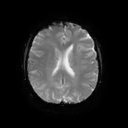
\includegraphics[scale=0.9,angle=0]{Im1.png}
    \caption{IRM sans produit de contraste.}
    \label{fig:without} 
\end{subfigure}
\begin{subfigure}[t]{0.3\textwidth}
\centering
    \vspace{0.00\textheight}
    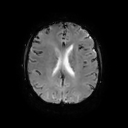
\includegraphics[scale=0.9,angle=0]{Im7.png}
    \caption{Début de la diffusion.}
    \label{fig:First} 
\end{subfigure}
\begin{subfigure}[t]{0.3\textwidth}
\centering
    \vspace{0.00\textheight}
    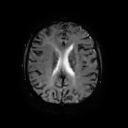
\includegraphics[scale=0.9,angle=0]{Im8.png}
    \caption{Pic de diffusion.}
    \label{fig:Second} 
\end{subfigure}
\begin{subfigure}[t]{0.3\textwidth}
\centering
    \vspace{0.00\textheight}
    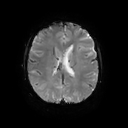
\includegraphics[scale=0.9,angle=0]{Im13.png}
    \caption{Fin de la diffusion.}
    \label{fig:Last} 
\end{subfigure}
    \caption{Diffusion du produit de contraste dans une IRM de perfusion.}
    \label{fig:diffusion} 
\end{figure}

Pour chacune des IRM de cerveau que nous avons récupéré, nous avons donc obtenu un ensemble d'images IRM qui sont réparties selon 24 ou 26 coupes avec pour chaque coupe 40 images traduisant la diffusion du produit de contraste et chaque image est de dimension 256 sur 256 pixels. On a donc pour chaque coupe un tenseur de dimension 256*256*40 qui contient toutes les informations sur la diffusion du produit de contraste.

\medskip

Quelque soit l'IRM considérée, la chaine de traitement restera la même. Il faudra choisir l'IRM d'un patient, stocker les images IRMs par coupe, choisir une coupe puis une région d'intérêt et enfin appliquer l'algorithme sur les éléments sélectionnés comme le montre la figure \ref{fig:toolchain}.


\begin{figure}[H]
\centering
    \includegraphics[scale=0.8,angle=0]{Images/Processing_toolchain.png}
    \caption{Chaine de traitement développée dans le cadre du projet.}
    \label{fig:toolchain}
\end{figure}


La sélection de la région d'intérêt se fait assez facilement avec Matlab comme le montre la figure suivante. L'idée est de prendre une zone et une coupe qui contiennent la zone présentant une pathologie. La partie qui suit va donc consister à expliquer comment on peut, à partir des signaux d'intensité de chacun des pixels, réaliser des clusters qui représentent des tissus homogènes et qui ont donc le même comportement pendant la diffusion du produit de contraste.

\begin{figure}[H]
\centering
    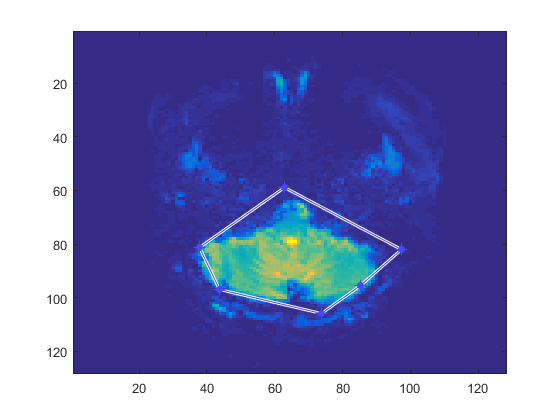
\includegraphics[scale=0.8,angle=0]{Images/ExampleROI.png}
    \caption{Choix d'une région d'intérêt avec Matlab.}
    \label{fig:ExampleROI}
\end{figure}



\chapter{Intérêt de la classification spectrale.}

Il existe une très large bibliographie sur la classification non supervisée. Néanmoins, comme le montre la figure suivante, l'algorithme du K-means ne parvient pas à aboutir au résultat escompté. 

\begin{figure}[H]
\centering
\begin{subfigure}[t]{0.6\textwidth}
\centering
    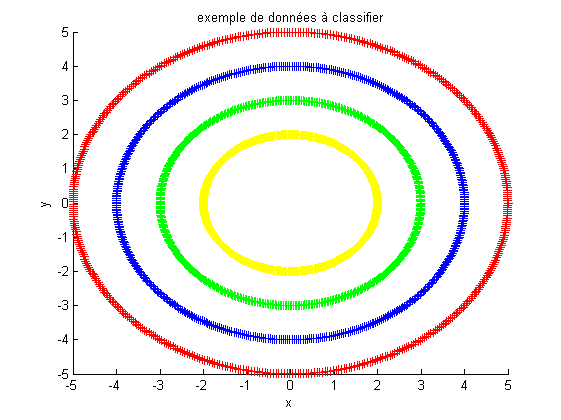
\includegraphics[scale=0.6,angle=0]{Images/DataSet.png}
    \caption{Ensemble de données de départ. Les données sont générées sur un cercle dont le rayon varie selon la classe}
    \label{fig:DataSet}
\end{subfigure}
\begin{subfigure}[t]{0.6\textwidth}
\centering
    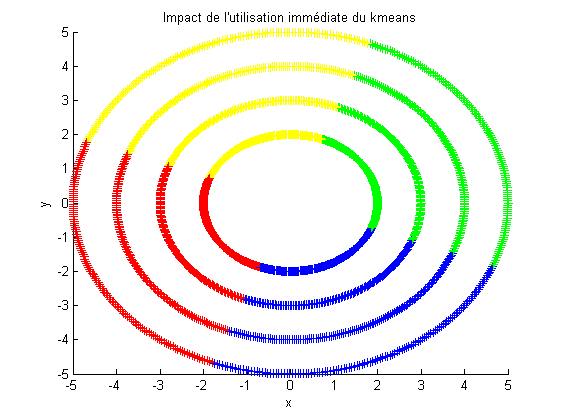
\includegraphics[scale=0.6,angle=0]{Images/AlgoKmeans.png}
    \caption{Application du Kmeans sur cet ensemble de données. Les données ne sont pas correctement classifiées.}
    \label{fig:AlgoKmeans}
\end{subfigure}
\end{figure}

Ici, tous les nuages de points présentent un même centre et cela fausse le résultat bien que des zones de frontières sont facilement identifiables. L'intérêt de la classification spectrale est de construire un graphe par l'intermédiaire d'une matrice de voisinage qui va traduire les similitudes entre les entrées. Ensuite, il faut travailler sur le spectre de cette matrice afin de pouvoir faire une classification. 

\medskip

Dans notre cas d'étude, nous devons étudier des signaux temporels dont on ne connait a priori aucuns paramètres discriminants. Il est donc nécessaire de parvenir à trouver un espace dans lequel la classification puisse aboutir à des résultats pertinents. La classification spectrale est donc ici particulièrement adaptée par rapport aux autres algorithmes de classification non supervisé.

\chapter{Choix réalisé pour l'implémentation de la classification spectrale.}

Nous devions implémenter un algorithme qui puisse être assez robuste pour traiter différents types d'informations, que ce soit les intensités des pixels des images IRM que nous étudions que des données simulées quelconques. C'est pour cela que certains choix dans la mise en place de l'algorithme ont été fait. Le lecteur pourra trouver en annexe des informations sur la théorie des graphes et également une partie des algorithmes qui ont été développés mais qui n'ont pas servis dans la chaine de traitement finale.

Une fois que l'opérateur a sélectionné une région d'intérêt, on génère une matrice qui contient les courbes d'intensité des pixels sélectionnés. Cette matrice est donnée en entrée de notre chaine de traitement comme le montre la figure \ref{fig:toolchain}.

\section{Choix dans la construction du graphe et de la matrice de similitude.}

Nous voulions avoir une chaine de traitement qui soit la plus robuste et la plus automatisée possible. Nous n'avons aucune connaissance a priori sur les données en entrée donc il faut calculer un coefficient de similitude entre toutes les données entre elles. Par conséquent, on a choisi de construire un graphe entièrement connecté ce qui se traduit par l' attribution d'un coefficient de similitude $W_{ij} = W_{ji}$ pour les signaux du pixel $i$ et du pixel $j$.  

\medskip

On va donc représenter notre graphe par une matrice de similitude W qui aura comme propriété d'être symétrique. Chaque nœud du graphe correspondra à une ligne ou une colonne de la matrice et le coefficient $W_{ij}$ correspondra au lien reliant les nœuds $i$ et $j$. Il faut après définir le coefficient de similitude $W_{ij}$. L'annexe E contient les différentes définitions qui peuvent être choisies. Celle qui donne le plus satisfaction est la similitude euclidienne qui est définie par: 

\medskip


\begin{equation}
W_{ij} = exp(-\frac{d^2(x_i,x_j)}{2\sigma_i\sigma_j})
\end{equation} 

\medskip


Où $x_i$ est le signal du pixel $i$, $\sigma_i$ est un paramètre qui traduit la dispersion des entrées autour de $x_i$ et $d(x_i,x_j)$ est la distance euclidienne entre les signaux $x_i$ et $x_j$. Le document \cite{mouysset2010contributions} donne plusieurs définitions pour ce paramètre et la définition qui donne le plus satisfaction est de prendre $\sigma_i = d(x_i,x_r)$ où $x_r$ correspond au septième voisin le pus proche de $x_i$. 

\medskip


Au final, nous arrivons à une matrice de similitude comme celle ci-dessous pour des données réelles. Cette dernière est affichée en fausse couleur. Les données qui ont été utilisées sont issues d'une IRM de cerveau où on a demandé une classification en 4 classes. La première figure montre la matrice d'affinité une fois tous les calculs réalisés et la seconde montre la matrice d'affinité après l'utilisation de notre algorithme de classification spectrale. On voit nettement 4 blocs au niveau de la diagonal de la matrice. Ces blocs traduisent que les données constitue une classe homogène. Les blocs hors-diagonaux traduisent la ressemblance interclasse. 

\begin{figure}[H]
\centering
    \includegraphics[scale=0.45,angle=0]{Images/MatrixAffinity2.png}
    \caption{Exemple de matrice de similitude.}
    \label{fig:MatrixAffinity2}
\end{figure}


\begin{figure}[H]
\centering
    \includegraphics[scale=0.45,angle=0]{Images/MatrixAffinity.png}
    \caption{Matrice de similitude après utilisation de l'algorithme de classification spectrale.}
    \label{fig:MatrixAffinity}
\end{figure}

Le dernière chose à faire est de définir le laplacien $L$ de la matrice $W$. Pour notre algorithme, nous utilisons le laplacien normalisée symétrique  $L $ défini par:

\begin{equation}
L = I-D^{-1/2}WD^{-1/2}
\end{equation}

Où la matrice $D$, matrice diagonale, contient les degrés des nœuds du graphe. Le degré d'un nœud est défini par $d_i = \Sigma_{v_j \in V} W_{ij}$. Et $I$ est la matrice identité.



\section{Choix de l'algorithme de classification spectrale.}

L'annexe G contient les algorithmes qui ont été implémentés durant le PFE. Pour chacun d'entre eux le principe reste le même. Il faut extraire des informations du spectre de la matrice Laplacienne du graphe qui a été construit avec les remarques ci-dessus. Dans un premier temps, on extrait les plus petites valeurs propres de la matrice L et les vecteurs associés. Ensuite, on applique un algorithme des k-means sur les données générées par la matrice qui contient les précédents vecteurs propres. Il y a plusieurs algorithmes de classification spectrale dans la littérature \cite{mouysset2010contributions} mais l'algorithme de Jordan et Weiss est celui qui nous a donné les meilleurs résultats. Les principales étapes sont données ci-dessous.

\begin{algorithm}[H]
  \caption{Normalized spectral clustering, Jordan and Weiss }
  
  \textbf{Entrées}% Inputs section
  \begin{algorithmic}[1]
    \STATE Matrice $W$ matrice de voisinage
    \STATE Entier $k$ nombre de classe
  \end{algorithmic}
  \bigskip

  \textbf{Sorties}% Output section
  \begin{algorithmic}[1]
    \STATE Vecteur $Ver$ table de vérité calculée.
  \end{algorithmic}
  \bigskip
  
  \textbf{Algorithme}
  \begin{algorithmic}[1]
		\STATE $L\gets$ Laplacien symétrique de la matrice $W$
     	\STATE $VectP\gets$ matrice contenant les vecteurs propres des k plus petites valeurs propres non nulles de L
     	\STATE normaliser toutes les lignes de la matrice $VectP$
     	\STATE $Ver\gets$ résultat de l'algorithme du Kmeans sur la matrice VectP en k clusters.	
  \RETURN $Ver$
  \end{algorithmic}
\end{algorithm}

\section{Choix du nombre de classe.}

Pendant cette étude, plusieurs méthodes ont été implémentées pour trouver automatiquement le nombre optimal de classe en fonction des données d'entrée. Le lecteur trouvera dans l'annexe C quelques algorithmes qui peuvent être utilisés. Sur les données réelles, aucuns d'entre eux ont donné de résultat. Par conséquent, l'opérateur qui utilisera notre algorithme et notre chaine de traitement devra tout de même donner le nombre de classe qu'il souhaite générer. 

\medskip

Au final, notre chaine de traitement a besoin de deux éléments:

\begin{itemize}
\item Une zone d'intérêt ou ROI qui doit être sélectionnée par l'opérateur. Ce qui suppose néanmoins une connaissance a priori sur la zone à étudier.
\item Le nombre de cluster souhaité car il ne peut être trouver de manière automatique.
\end{itemize}

\chapter{Résultats de l'algorithme et interprétations.}


Nous avons dans un premier temps utilisé notre algorithme sur des données simples comme celle qui est utilisé dans le chapitre 5. Voici le résultat que nous obtenons après l'utilisation de l'algorithme que nous avons expliqué dans la partie précédente.

\begin{figure}[H]
\centering
    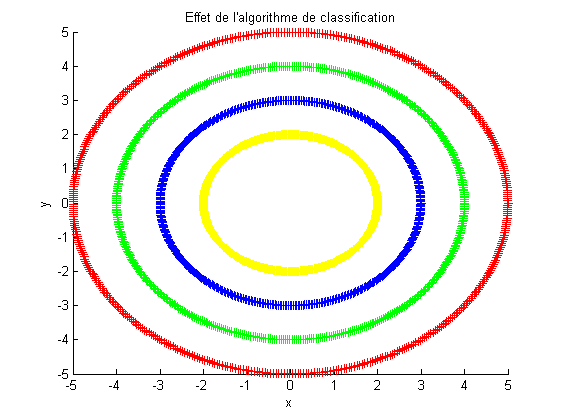
\includegraphics[scale=0.6,angle=0]{Images/AlgoClssification.png}
    \caption{Application du premier algorithme sur les premières données. Les données sont correctement classifiées.}
    \label{fig:AlgoClssification}
\end{figure}

On peut voir que le résultat obtenu est bien celui espéré et que c'est une solution parfaitement viable pour agréger des données dans des clusters bien que les liens entre elles ne soient pas identifiable immédiatement. Les valeurs propres extraites du laplacien et qui sont utilisées pour la classification sont données ci-dessous.

\begin{figure}[H]
\centering
    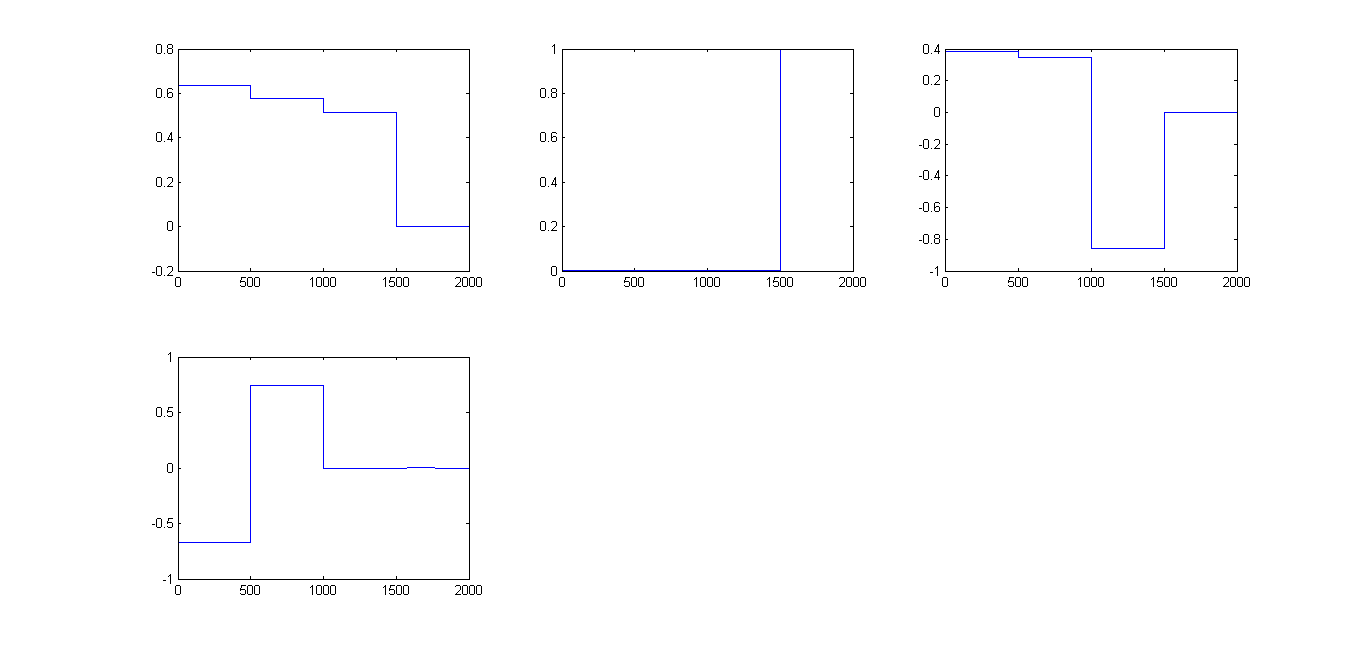
\includegraphics[scale=0.4,angle=0]{Images/VecteursPropres.png}
    \caption{Vecteurs propres extraits du laplacien.}
    \label{fig:VecteursPropres}
\end{figure}

On peut clairement voir comment les K-means, sur ces données extraites, permettent des discriminer les quatre classes. Nous l'avons testé sur un ensemble de test et les figures suivantes montrent les résultats que nous avons obtenu.


\begin{figure}[H]
\centering
    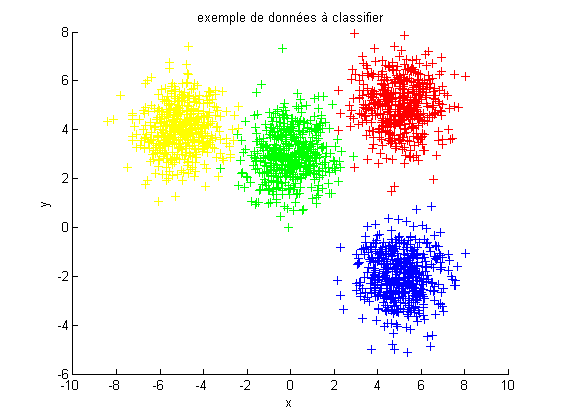
\includegraphics[scale=0.6,angle=0]{Images/DataSet2.png}
    \caption{Second ensemble de données.}
    \label{fig:DataSet2}
\end{figure}

\begin{figure}[H]
\centering
    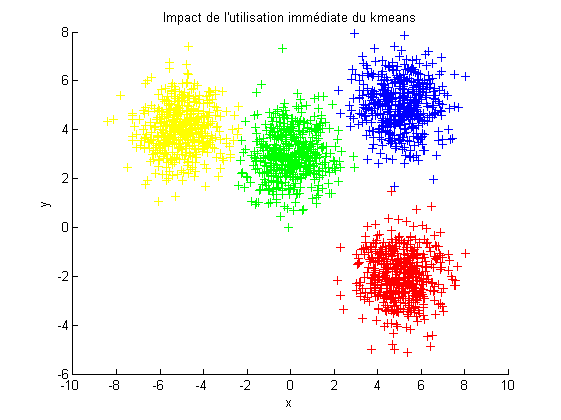
\includegraphics[scale=0.6,angle=0]{Images/AlgoKmeans2.png}
    \caption{Application du Kmeans sur le second ensemble de données.}
    \label{fig:AlgoKmeans2}
\end{figure}

\begin{figure}[H]
\centering
    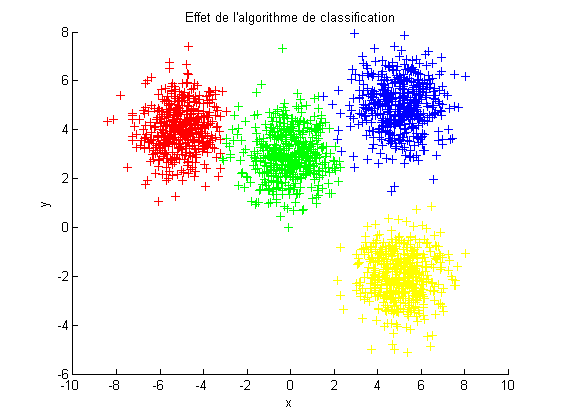
\includegraphics[scale=0.6,angle=0]{Images/AlgoClssification2.png}
    \caption{Application du premier algorithme sur le second ensemble de données.}
    \label{fig:AlgoClssification2}
\end{figure}

\begin{figure}[H]
\centering
    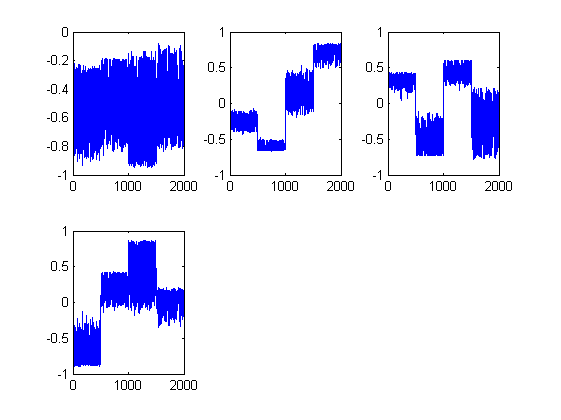
\includegraphics[scale=0.4,angle=0]{Images/VecteursPropres2.png}
    \caption{Vecteurs propres extraits du laplacien.}
    \label{fig:VecteursPropres2}
\end{figure}

Là encore, le résultat est très satisfaisant.


\chapter*{Conclusion}

Au terme de cette étude, nous pouvons extraire ces différents résultats:

\begin{itemize}
\item Tout d'abord, la classification spectrale est particulièrement adaptée pour les problèmes que les algorithmes traditionnels comme le K-means ne peuvent résoudre. On arrive à se placer facilement dans un nouvel espace qui permet d'identifier clairement les éléments appartenant à une même classe. Il est donc tout à fait pertinent pour les signaux que nous devons traiter.
\item La mise en place des différents algorithmes est au final relativement simple et peut couteuse en temps de calcul. Néanmoins, si le nombre de point devient trop grand, il peut y avoir un problème sur le temps d'exécution.
\item La chaine de traitement qui a été développé est très robuste et peut fonctionner dans beaucoup de cas étant donné que nous ne faisons pas d'apriori sur les données de départ et que nous calculons les similitudes de toutes les entrées entre elles.
\end{itemize}

\medskip

Néanmoins, il y a plusieurs contraintes qui faut prendre en compte:

\begin{itemize}
\item Le résultat final est fortement impacté par l'utilisation du K-means à la fin de l'algorithme de classification spectrale. Il arrive que l'algorithme ne converge pas vers les solutions souhaitées en fonction de l'initialisation.
\item Il y a un besoin de connaissance a priori sur le nombre de classe que nous souhaitons. Cela veut dire que notre chaine de traitement ne pourra pas être entièrement autonome.
\end{itemize}